% !TEX TS-program = pdflatex
% !TEX encoding = UTF-8 Unicode

% TO COMPILE: lmake (animal scrifices may be necessary)
%%%%%%%%%%%%%%%%%%%%%%%%%%%%%%%%%%%%%%%%%%%%%%%%%%%%%%%%%%%%%%%%%%%%%%%%%%
%																							                           %
%				                         PREAMBLE      							             %
%                                                                        %
%%%%%%%%%%%%%%%%%%%%%%%%%%%%%%%%%%%%%%%%%%%%%%%%%%%%%%%%%%%%%%%%%%%%%%%%%%
\documentclass[compress]{beamer}

\mode<presentation>
{
  \usetheme{Frankfurt}
  \usecolortheme{crane}
  \setbeamercovered{transparent}
}

% Package Setup
%%%%%%%%%%%%%%%%%%%%%%%%%%%%%%%%%%%%%%%%%%%%%%%%%%%%%%%%%%%%%%%%%%%%%%%%%%
%                                                                        %
%                                 PREAMBLE                               %
%                                                                        %
%%%%%%%%%%%%%%%%%%%%%%%%%%%%%%%%%%%%%%%%%%%%%%%%%%%%%%%%%%%%%%%%%%%%%%%%%%

%% PACKAGES
\usepackage[]{lineno}
\usepackage{fancyvrb}
%\linenumbers
\usepackage{amsmath}
\usepackage{microtype}
\usepackage{algorithmic}

%% GRAPHICS RELATED
\usepackage{graphicx}
\usepackage[outdir=./tmp/]{epstopdf}
\graphicspath{{../images/}{./}{./tmp/}}
\DeclareGraphicsExtensions{.eps, .pdf, .jpeg, .png}

%% CAPTION SETUP
\usepackage{float}
\usepackage[font=footnotesize]{caption}
\usepackage[font=small]{subcaption}
\captionsetup{belowskip=12pt,aboveskip=4pt}

%% BEAMER
\usepackage{multicol}
\usepackage{multirow}
\usepackage{array}				% Table Stuff
\usepackage{arydshln}
\usepackage{rotating}

%% BIBLIOGRAPHY
\bibliographystyle{ieeetr}

%% UNITS
\usepackage{siunitx}

%% EQUATIONS
%\numberwithin{equation}{section}

%%%%%%%%%%%%%%%%%%%%%%%%%%%%%%%%%%%%%%%%%%%%%%%%%%%%%%%%%%%%%%%%%%%%%%%%%%%
%                                                                         %
%                             Listing Setup                               %
%                                                                         %
%%%%%%%%%%%%%%%%%%%%%%%%%%%%%%%%%%%%%%%%%%%%%%%%%%%%%%%%%%%%%%%%%%%%%%%%%%%
\usepackage{listings}
\lstset{ %
    language=C++,
    basicstyle=\footnotesize\ttfamily,
    numbers=left,
    numberstyle=\tiny\color{gray},
    stepnumber=2,
    numbersep=5pt,
    backgroundcolor=\color{white},
    showspaces=false,
    showstringspaces=false,
    showtabs=false,
    frame=single,
    rulecolor=\color{black},
    tabsize=2,
    breaklines=true,
    breakatwhitespace=false,
    title=\lstname,
    keywordstyle=\color{blue},
    commentstyle=\color{OliveGreen},
    stringstyle=\color{orange}
}
\DeclareCaptionFont{white}{\color{white}}
\DeclareCaptionFormat{listing}{\colorbox[cmyk]{0.43, 0.35, 0.35, 0.01}{\parbox{\dimexpr\textwidth-2\fboxsep\relax}{#1#2#3}}}
\captionsetup[lstlisting]{format=listing,labelfont=white,textfont=white,singlelinecheck=false,margin=0pt,font={bf,footnotesize}}
%\lstnewenvironment{code}[1][]%
%{ \noindent\minipage{\linewidth}
%	\lstset{#1}
%}
%{\endminipage}
%% USER COMMANDS
\usepackage{isotope}
\newcommand{\iso}{\isotope}
\newcommand{\figurewidth}{\textwidth}
\newcommand{\micron}{$\mu$m}



% Preamble / Frst Size
%\setbeamersize{text margin left=5mm, text margin right 5mm}
\title[Turner Symposium] {Monte Carlo Single Collision Energy Loss Spectra in Water}
\author[] {
    Matthew Urffer\inst{1}
}
\institute[University of Tennessee] { 
  \inst{1}%
  Department of Nuclear Engineering,
  University of Tennessee, Knoxville, TN
}

\date[] {May 22-23, 2013}
\pgfdeclareimage[height=0.5cm]{university-logo}{../../images/utwordmarkhorz.png}
\logo{\pgfuseimage{university-logo}}

\begin{document}

\begin{frame}[plain]
  \titlepage
  \tiny
    \begin{center}
\centering{Financial support from the Domestic Nuclear Detection Office (DNDO) through Award No. 003387891 is gratefully acknowledged. 
  Any opinions, findings, and conclusions or recommendations expressed in this material are those of the presenter and do not necessarily reflect the views of DNDO.}
  \end{center}
\end{frame}

\begin{frame}{Table of Contents}
  \begin{multicols}{2}
    \tableofcontents
  \end{multicols}
\end{frame}


%%%%%%%%%%%%%%%%%%%%%%%%%%%%%%%%%%%%%%%%%%%%%%%%%%%%%%%%%%%%%%%%%%%%%%%%%%
%                                                                        %
%                            INTRODUCTION                                %
%                                                                        %
%%%%%%%%%%%%%%%%%%%%%%%%%%%%%%%%%%%%%%%%%%%%%%%%%%%%%%%%%%%%%%%%%%%%%%%%%%
\section{Introduction}
\subsection{Motivation}
%%%%%%%%%%%%%%%%%%%%%%%%%%%%%%%%%%%%%%%%%%%%%%%%%%%%%%%%%%%%%%%%%%%%%%%%%%
\begin{frame}[fragile]{Motivation}
  Biological:
  \begin{itemize}
  \item Fundamental to understanding low energy electrons interactions with matter
  \item Low energy electrons produce the inital chemical changes in tissue and tissue like material (water)
  \end{itemize}
  Secondary Electron Range Calculations:
  \begin{itemize}
    \item Low energy, high fidelity low energy electron transport needed for gamma discrimination simulation
    \item GEANT4 (with \verb+G4DNAPhysics+) provide the ability to simulate low energy electron interactions
    \item Ability to validate GEANT4 simulation
  \end{itemize}
\end{frame}
%%%%%%%%%%%%%%%%%%%%%%%%%%%%%%%%%%%%%%%%%%%%%%%%%%%%%%%%%%%%%%%%%%%%%%%%%%
\begin{frame}{Single Collision Energy Loss}
How much energy does an electron lose in a collision?
  \newtheorem{thm1}{Single Collision Energy Loss Defination}
  \begin{thm1}<1->
    \small
    Interaction of an electron of kinetic energy E with water can be described by the probability $N(E,E')dE$ that it loses an amount of energy between $E'$ and $E'+dE$
  \end{thm1}
  \begin{itemize}
    \item $N(E,E')$ is the single collision spectrum of $E$
    \item $N(E,E')$ is a normalized probability function
  \end{itemize}
\end{frame}
%%%%%%%%%%%%%%%%%%%%%%%%%%%%%%%%%%%%%%%%%%%%%%%%%%%%%%%%%%%%%%%%%%%%%%%%%%
\subsection{Turner Ties}
\begin{frame}{Historical Ties to Turner}
  \begin{itemize}
    \item Original work was completed by Turner in 1982
    \item Results were later included in Atoms, Radiation, and Radiation Protection
  \end{itemize}
    \begin{figure}
      \centering
      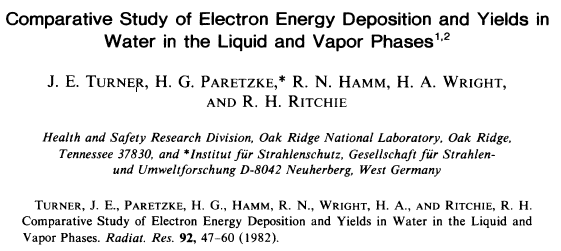
\includegraphics[width=0.75\textheight]{TurnerArticleHeading}
    \end{figure}
\end{frame}
%%%%%%%%%%%%%%%%%%%%%%%%%%%%%%%%%%%%%%%%%%%%%%%%%%%%%%%%%%%%%%%%%%%%%%%%%%
\begin{frame}{Project Goal}
  \centering
  Simualtion goal is to reproduce Turner's figure
  \begin{figure}
    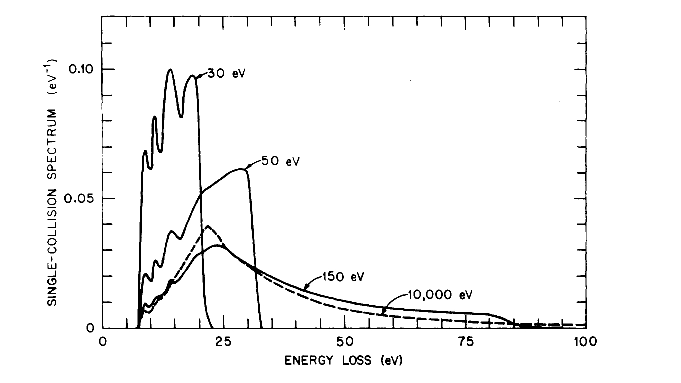
\includegraphics[width=0.6\textwidth]{Turner_Fig2_SingleCollisionELoss}
  \end{figure}
  \flushleft
  Example:
  \begin{itemize}
    \small
    \item For \SI{10}{\keV}, the average value of the single collision energy loss between \SI{45}{\keV} to \SI{50}{\keV} is 0.1 $\text{eV}^{-1}$
    \item Interval is \SI{5}{\keV}, so 5\% chance that a \SI{10}{\keV} electron in water has an energy loss between \SI{45}{\keV} and \SI{50}{\keV} in it's first collision
  \end{itemize}
\end{frame}
%%%%%%%%%%%%%%%%%%%%%%%%%%%%%%%%%%%%%%%%%%%%%%%%%%%%%%%%%%%%%%%%%%%%%%%%%%
%                                                                        %
%                                METHODS                                 %
%                                                                        %
%%%%%%%%%%%%%%%%%%%%%%%%%%%%%%%%%%%%%%%%%%%%%%%%%%%%%%%%%%%%%%%%%%%%%%%%%%
\section{Methods}
\subsection{GEANT4}
\begin{frame}[fragile]{GEANT4 Introduction}
What GEANT4 is:
\begin{itemize}
  \small
  \item \href{geant4.cern.ch}{geant4.cern.ch}
  \item Free software package for the simulation of the passage of particles through matter
  \item Essentially a collection of tools for geometry, materials, physics models, events and digitilization, visulations $\dots$
  \item Maintained by the CERN community, widely used in physics
\end{itemize}
What GEANT4 is not:
\begin{itemize}
  \small
  \item For the timid
  \begin{itemize}
    \item Users are responsible for correctly implementing their own physics
    \item Users are responsible for correctly implementing their own analysis
  \end{itemize}
  \item Stagnat - major release are still occuring
\end{itemize}
\end{frame}
%%%%%%%%%%%%%%%%%%%%%%%%%%%%%%%%%%%%%%%%%%%%%%%%%%%%%%%%%%%%%%%%%%%%%%%%%%
\begin{frame}[fragile]{GEANT4 Microdose Models}
\verb+G4DNAPhyscis+, \href{geant4-dna.in2p3.fr}{geant4-dna.in2p3.fr/index.html}
  \begin{itemize}
    \item A microdose model for modeling early biological damage by ionizing radiation on the DNA scale
    \item Electron interactions include: elastic scattering (\SI{7.4}{\eV}), electronic excitation (\SI{9}{\eV}), ionisation (\SI{11}{\eV}), vibrational excitation (\SI{2}{\eV})
    \item Similar methods exist for the protons, alphas
    \item Only material defined is \verb+G4_WATER+ (NIST based)
  \end{itemize}
\end{frame}
%%%%%%%%%%%%%%%%%%%%%%%%%%%%%%%%%%%%%%%%%%%%%%%%%%%%%%%%%%%%%%%%%%%%%%%%%%
\begin{frame}[fragile]{Implemented Simulation}
  \begin{columns}[onlytextwidth]
    \begin{column}{0.45\textwidth}
      \begin{itemize}
         \item Electrons shot into a cube of water
         \item Intial events chosen by a particle gun
         \item Verbose tracking for first change in energy, in addition to bining on this value through ROOT
      \end{itemize}
    \end{column}
    \begin{column}{0.45\textwidth}
      \begin{figure}
        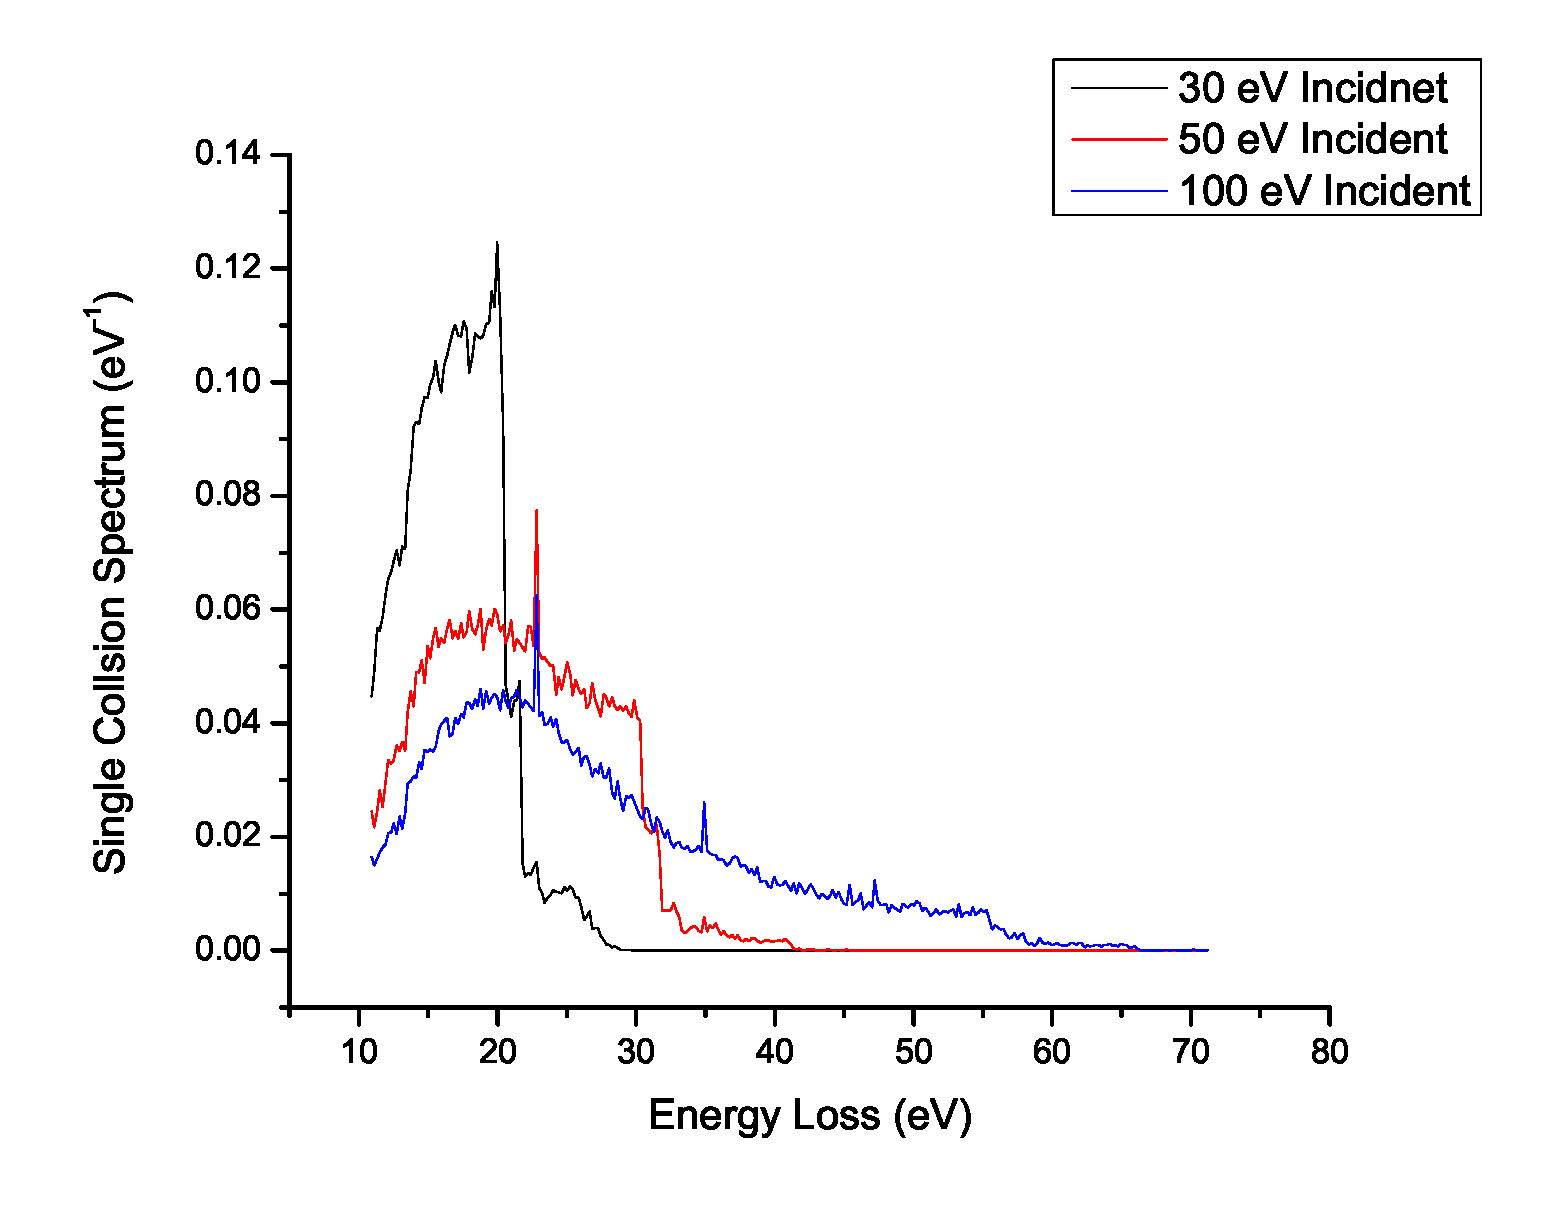
\includegraphics[width=\textwidth]{SingleCollisionEnergyLoss_300bins}
        \caption{Simulation and Track}
    \end{figure}
    \end{column}
  \end{columns}
\end{frame}
%%%%%%%%%%%%%%%%%%%%%%%%%%%%%%%%%%%%%%%%%%%%%%%%%%%%%%%%%%%%%%%%%%%%%%%%%%
%                                                                        %
%                               RESULTS                                  %
%                                                                        %
%%%%%%%%%%%%%%%%%%%%%%%%%%%%%%%%%%%%%%%%%%%%%%%%%%%%%%%%%%%%%%%%%%%%%%%%%%
\section{Results}
\begin{frame}{GEANT4 Single Collision Energy Loss}
  \begin{figure}
    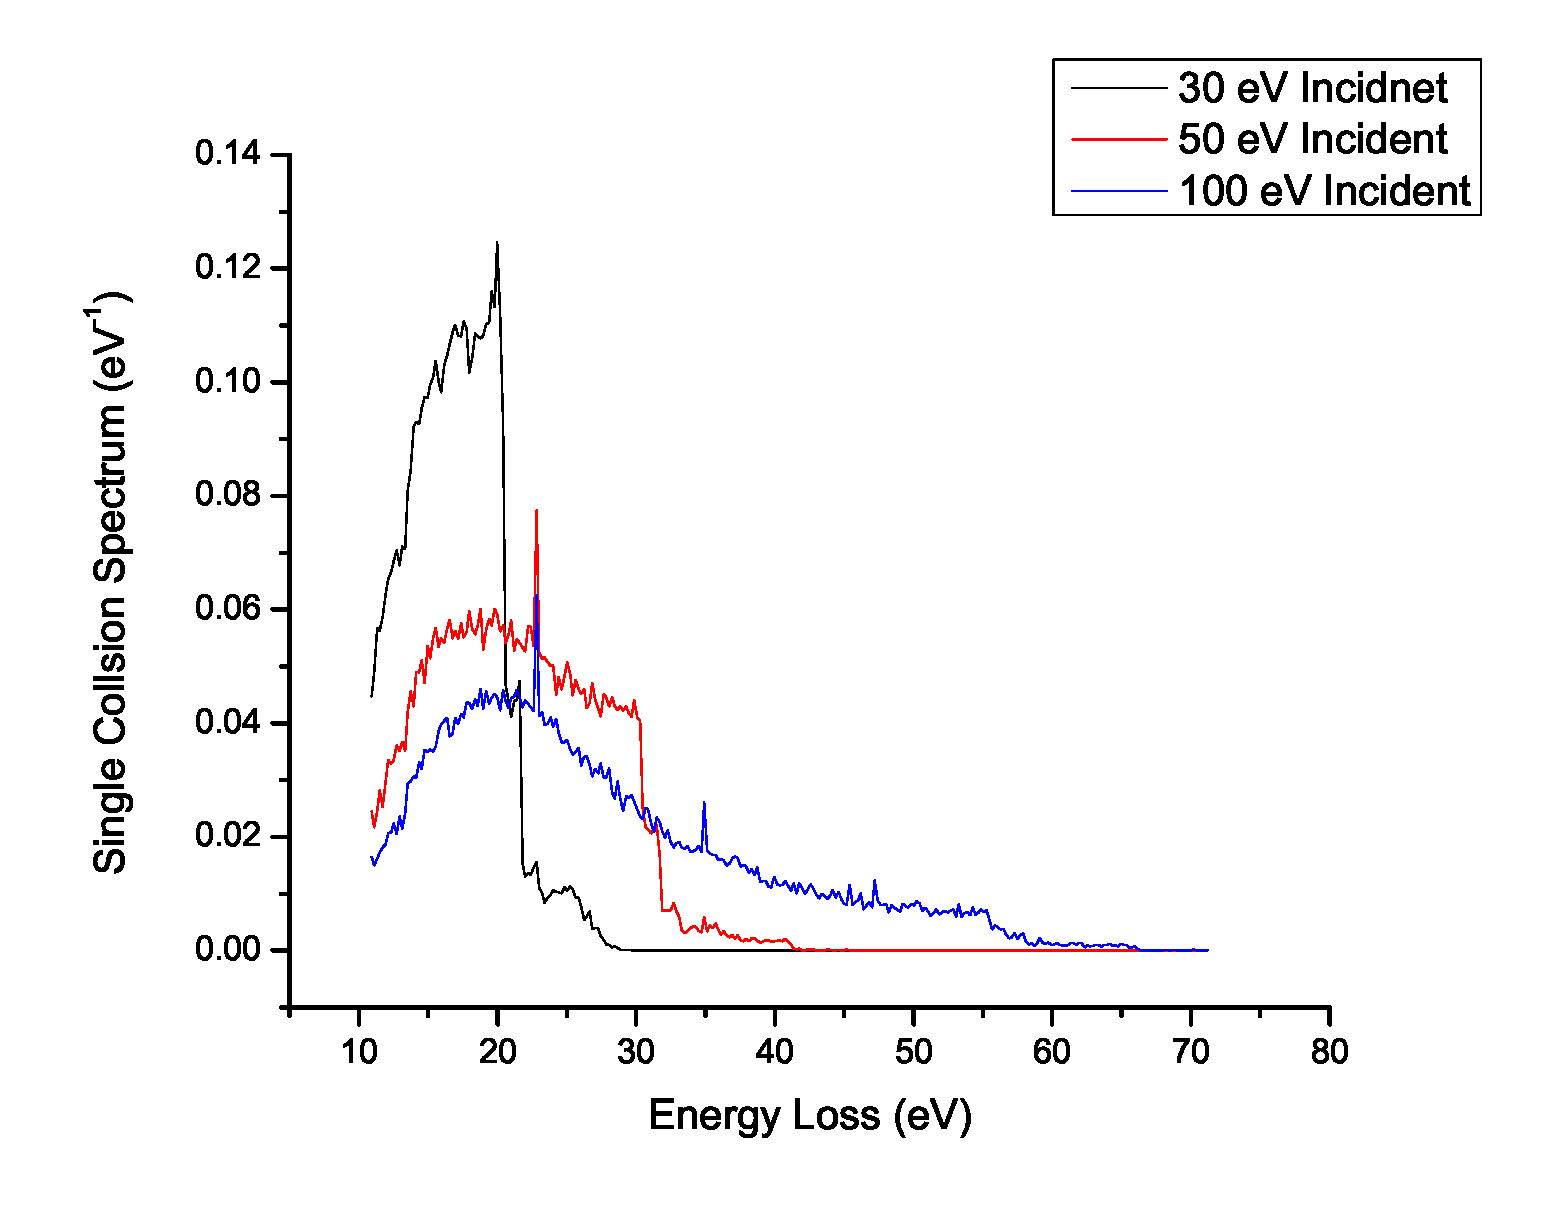
\includegraphics[width=0.75\textwidth]{SingleCollisionEnergyLoss_300bins}
  \end{figure}
\end{frame}
\begin{frame}{Comparison to Turner}
  \begin{columns}[onlytextwidth]
    \begin{column}{0.45\textwidth}
      \begin{figure}
        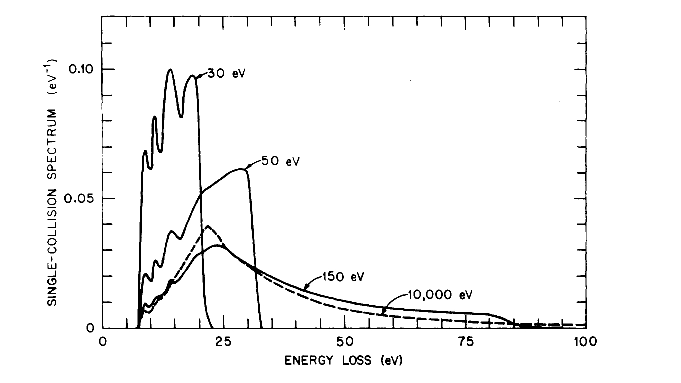
\includegraphics[width=\textwidth]{Turner_Fig2_SingleCollisionELoss}
        \caption{Tuner Spectrum}
      \end{figure}
    \end{column}
    \begin{column}{0.45\textwidth}
      \begin{figure}
        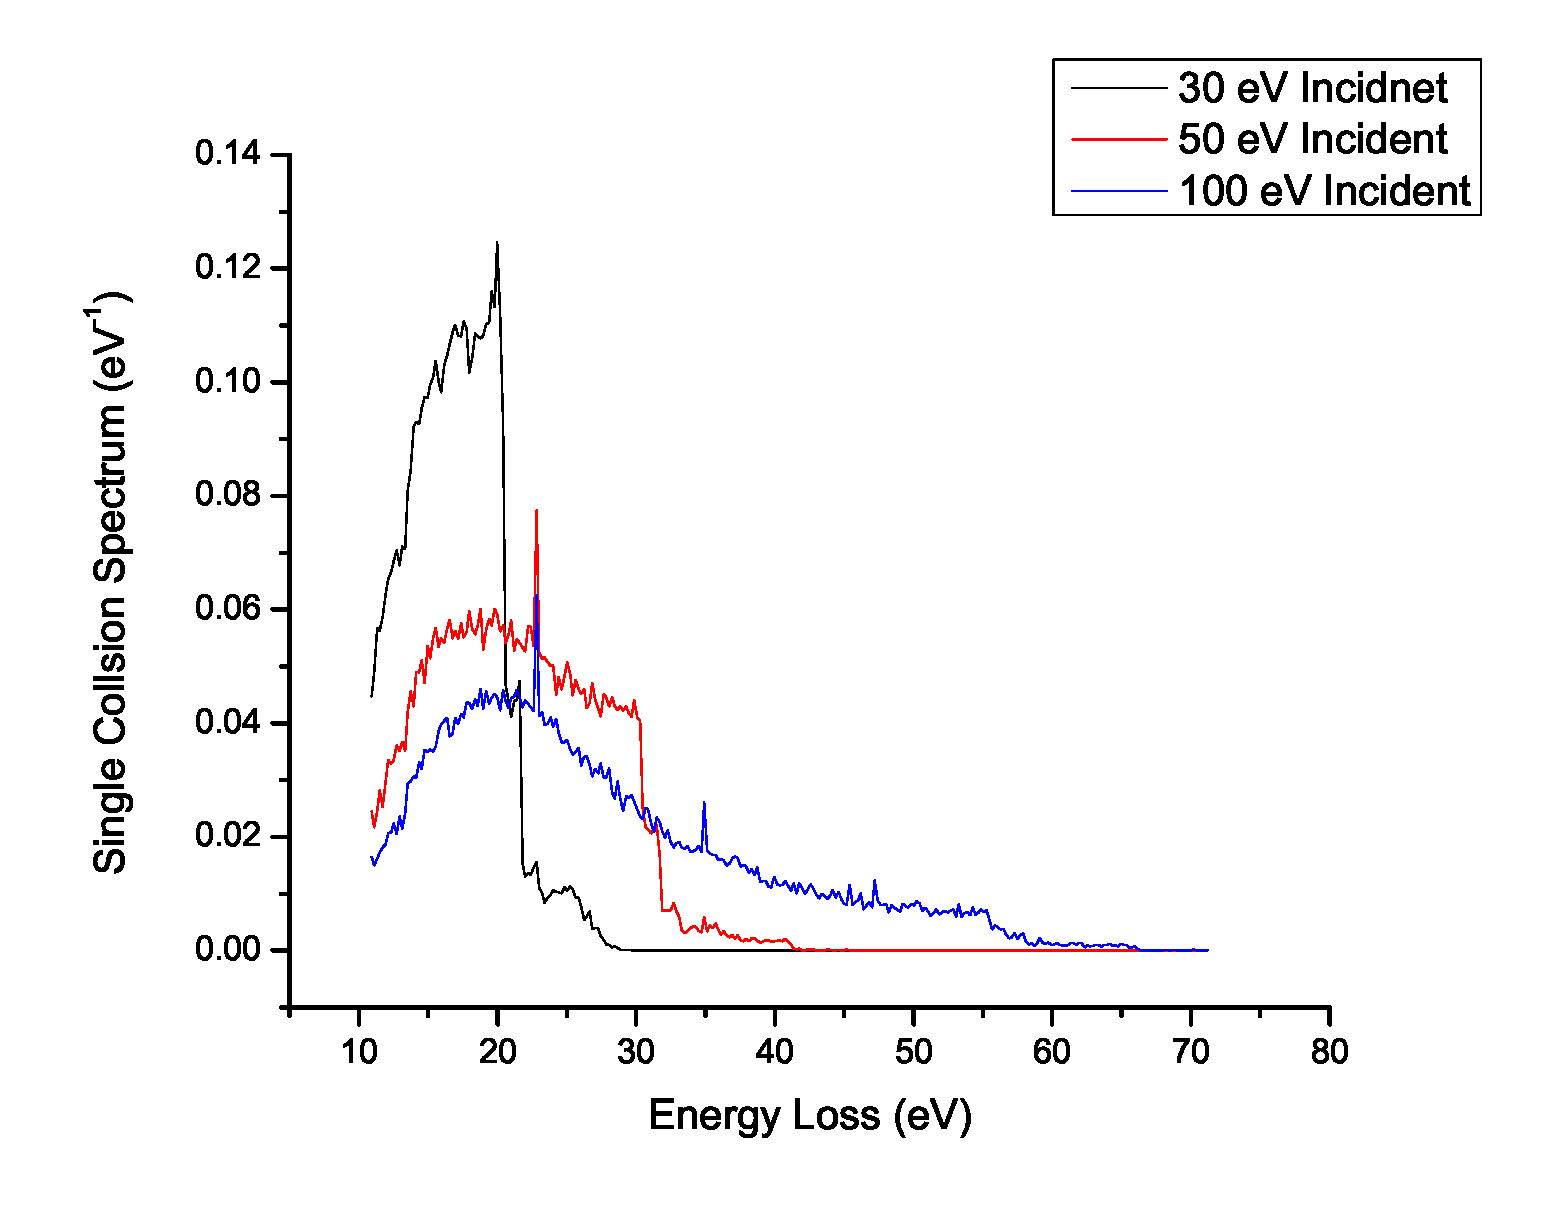
\includegraphics[width=\textwidth]{SingleCollisionEnergyLoss_300bins}
        \caption{GEANT4 Simulated Spectrum}
    \end{figure}
    \end{column}
  \end{columns}
\vspace{2mm}
Disgrepancies are in the resolution of cross section data
\end{frame}
%%%%%%%%%%%%%%%%%%%%%%%%%%%%%%%%%%%%%%%%%%%%%%%%%%%%%%%%%%%%%%%%%%%%%%%%%
\begin{frame}{Introduction}
	\begin{itemize}
		\item Brief Histroy of the Single Collision Energy Loss
		\item What is the single collision energy loss
		\item How the simulation was preformed
		\begin{itemize}
			\item Background of the simulation
			\item Maybe a track plotted
			\item Microdose physics
			\item How the energy loss was calcualted
		\end{itemize}
	\end{itemize}
\end{frame}
%%%%%%%%%%%%%%%%%%%%%%%%%%%%%%%%%%%%%%%%%%%%%%%%%%%%%%%%%%%%%%%%%%%%%%%%%%
%%%%%%%%%%%%%%%%%%%%%%%%%%%%%%%%%%%%%%%%%%%%%%%%%%%%%%%%%%%%%%%%%%%%%%%%%%
%                                                                        %
%                            CONCLUSIONS                                 %
%                                                                        %
%%%%%%%%%%%%%%%%%%%%%%%%%%%%%%%%%%%%%%%%%%%%%%%%%%%%%%%%%%%%%%%%%%%%%%%%%%
\begin{frame}{Summary}
  \begin{itemize}
    \item Successfully validated a GEANT4 simulation of the energy depostion of electrons in water
  \end{itemize}
\end{frame}
%%%%%%%%%%%%%%%%%%%%%%%%%%%%%%%%%%%%%%%%%%%%%%%%%%%%%%%%%%%%%%%%%%%%%%%%%%%
\begin{frame}
	\centering
  \begin{figure}
    
\includegraphics[height=8cm]{Questions.eps}
  \end{figure}
\end{frame}
%%%%%%%%%%%%%%%%%%%%%%%%%%%%%%%%%%%%%%%%%%%%%%%%%%%%%%%%%%%%%%%%%%%%%%%%%%%
% BILBIOLGRAPHY
%\begin{frame}[plain,allowframebreaks]
%\frametitle{Works Cited}
%	\tiny
%  \bibliography{../Zotero}
%\end{frame}

\end{document}


